
\chapter{Introducción}
\label{ch:intro}

En este primer capítulo, se presentarán a modo de introducción los aspectos más relevantes del \gls{tfm} desarrollado, como son la transformación de las redes energéticas en nuevas redes inteligentes de energía (del inglés \gls{sg}) y su consecuente necesidad de monitorización, además del creciente auge de la \gls{ia} y de las técnicas de aprendizaje automático y profundo (del inglés \gls{ml} y \gls{dl}).

\vspace{3mm}

De la misma manera, se hará hincapié en los objetivos que se establecen para este \gls{tfm}, describiendo así la secuencia de acciones que se seguirá para poder llevarlos a cabo. Dichos objetivos serán los pilares sobre los que se sustente el diseño y el desarrollo de modelos eficientes basado en \gls{ml} y \gls{dl} para la detección y predicción de errores en \gls{sg}s. De forma adicional, se incluirá un último apartado en referencia a la estructura de capítulos que seguirá este \gls{tfm}, así como una explicación breve sobre los temas que se abordarán en cada uno de ellos.


\section{Presentación}
\label{sec:presentacion}

En los últimos años, el concepto de red eléctrica convencional está siendo completamente transformado como resultado del creciente desarrollo de las \gls{sg}s \cite{repsol} \cite{impact}. La posibilidad de brindar a tiempo real una monitorización del proceso de distribución eléctrica y a su vez, integrar una participación activa del consumidor convierte a estas redes en uno de los pilares de la transición hacia la descarbonización. 

\vspace{3mm}

En este contexto, se ha convertido en un objetivo primordial el diseño de nuevos protocolos que provean un encaminamiento y una distribución energética eficientes. Es por ello que, desde el equipo de investigación NetIS de la \gls{uah} se ha desarrollado el algoritmo \gls{den2ne} \cite{den2ne}, con el fin de automatizar la gestión de los recursos en entornos del Internet de las Cosas (del inglés \gls{iot}), enfocándose especialmente en \gls{sg}s.  

\pagebreak

Teniendo esto en cuenta, se puede expresar que \gls{den2ne} pretende realizar una distribución óptima de los recursos energéticos de cada uno de los nodos que presenta una determinada topología de red para conseguir finalmente un balance a nivel global. Sin embargo, el algoritmo se encuentra actualmente con un desafío a afrontar, basado en la imperiosa necesidad de poder detectar y predecir de una forma precisa los posibles errores que se puedan producir en el proceso de distribución energética entre nodos. En caso de fallos en la red, \gls{den2ne} debería tener la capacidad de responder de una forma rápida y específica, pues es de vital importancia tomar acciones a nivel de distribución para evitar que los errores se agraven y escalen al resto de la red.

\vspace{3mm}

\section{Objetivos}
\label{sec:obj}

Tomando en consideración el apartado anterior, se define como objetivo principal de este \gls{tfm} el desarrollo de diversas técnicas de \gls{ml} y \gls{dl} para identificar de forma precisa los posibles errores que se pueden producir en una \gls{sg} durante el proceso de distribución energética que, como se ha introducido, se aplicará mediante el algoritmo \gls{den2ne}. 

\vspace{3mm}

En otros términos, la identificación de patrones se apoyará en el análisis de grandes volúmenes de datos provenientes de implementaciones de \gls{sg}s reales. Estos serán previamente procesados de una forma exhaustiva para reducir su tamaño y seleccionar la información verdaderamente necesaria para el posterior desarrollo de los modelos. En la Figura \ref{fig:intro} se determina el diagrama de flujo que define la secuencia de acciones a realizar en este \gls{tfm}.

\vspace{4mm}

\begin{figure}[h!]
    \centering
    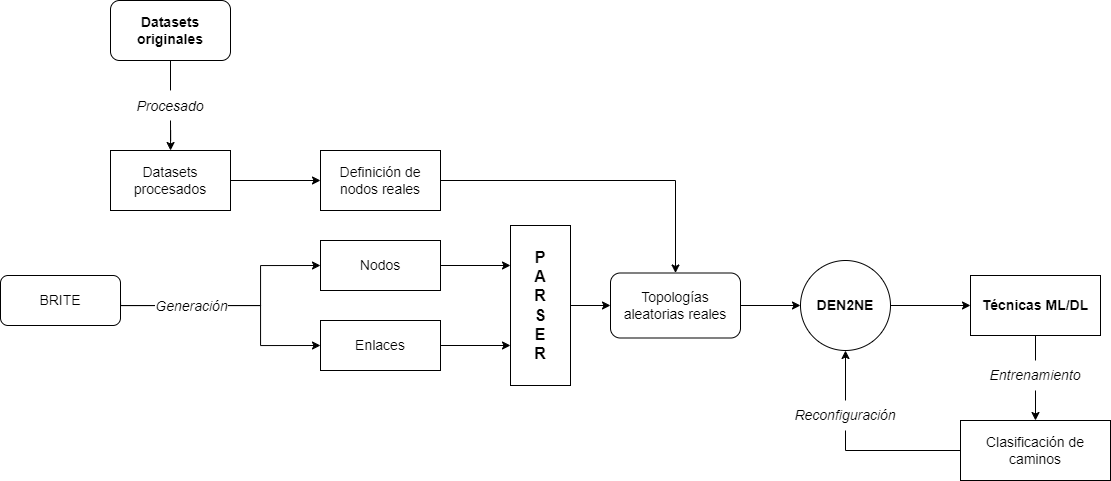
\includegraphics[width=1\textwidth]{img/intro/anteproyecto.drawio.png}
    \caption{Proceso de detección y predicción de errores}
    \label{fig:intro}
\end{figure}

\vspace{3mm}

\pagebreak

Por tanto, el presente \gls{tfm} permitirá determinar un modelo final de predicción de fallos para entornos de \gls{sg}s. Entrando en detalle, se pueden definir los diferentes objetivos en los siguientes puntos:

\begin{itemize}
    \item \textbf{Estudio del estado del arte y análisis de las diferentes fuentes de datos reales disponibles}. Se realizará un estudio en profundidad del contexto en el que se engloban las \gls{sg}s y los protocolos de distribución de recursos, poniendo el enfoque en \gls{den2ne}. Será necesaria una investigación sobre la disponibilidad de fuentes de datos reales y una evaluación de su viabilidad para este \gls{tfm}. De forma adicional, se precisará del estudio y análisis de herramientas de simulación de datos.
    
    \item \textbf{Definición y procesado del volumen de datos para el posterior desarrollo}. El procesamiento de los datos adquiridos será fundamental para simplificar su comprensión. Además, se llevará a cabo la selección de la cantidad de información realmente útil para el desarrollo.    

    \item \textbf{Planteamiento de escenarios y generación de diferentes topologías}. A partir del volumen final de datos que se elaborará, se plantearán una serie de escenarios mediante la generación de topologías de nodos con la herramienta BRITE \cite{brite}.
    
    \item \textbf{Simulación de topologías y extracción del conjunto de datos final}. Las topologías generadas se importarán a un simulador propietario realizado en python. Por consiguiente, se entrará en el funcionamiento del algoritmo \gls{den2ne} y se realizarán las modificaciones necesarias para que, mediante la ejecución del mismo, se pueda extraer el conjunto de datos final sobre el que se va a desarrollar.
    
    \item \textbf{Desarrollo y entrenamiento de diferentes modelos de \gls{ml} y \gls{dl}}. Se realizará un estudio sobre las posibles técnicas de \gls{ml} y \gls{dl} a emplear y se procederá a seleccionar las más apropiadas, según el contexto en el que se engloba este \gls{tfm}. Por consiguiente, se llevará a cabo el desarrollo y el entrenamiento de los mismos tomando como base los datos procesados anteriormente. 
    
    \item \textbf{Análisis y evaluación de los resultados obtenidos}. Se analizarán los resultados de detección y predicción de errores de los diferentes modelos desarrollados. Mediante el análisis en cuestión, se determinará de forma concluyente cuál aporta una mayor efectividad para poder diagnosticar con un alto porcentaje de precisión los errores que se producen en una \gls{sg}.
    
\end{itemize}

\section{Estructura del \glsentryshort{tfm}}
\label{sec:structure}

En esta sección se expone de forma general la estructura de capítulos que tendrá la memoria del presente \gls{tfm} con una breve descripción del contenido que abarcarán cada uno de ellos.

\begin{description}
    \item\textbf{Capítulo 1: Introducción}. Se comenzará esta memoria con una presentación de los aspectos más significativos. Se expondrán las motivaciones que han originado la realización de este \gls{tfm} y los objetivos que se prentenden alcanzar con el mismo.

    \item\textbf{Capítulo 2: Estado del arte}. Se establecerá el marco teórico en el que se sitúa este \gls{tfm} y se documentarán los conceptos principales para introducir en un contexto lo suficientemente consistente el diseño y desarrollo práctico posterior. Además, se expondrá de forma detallada el funcionamiento del algoritmo \gls{den2ne}.

    \item\textbf{Capítulo 3: Diseño y análisis de datos}. Se llevará a cabo un análisis sobre las posibilidades de diseño a través de una investigación exhaustiva sobre las fuentes de datos de implementaciones reales existentes, además de estudiar y ejecutar algunas herramientas de simulación para extraer información adicional. Después, se definirá todo el procesamiento que deberá llevarse a cabo sobre los datos para sintetizar los mismos y seleccionar únicamente la información útil. Las siguientes etapas vendrán definidas por el planteamiento de diferentes escenarios de red y la generación de topologías mediante la herramienta \gls{brite} y el algoritmo {den2ne}, respectivamente. Finalmente, se obtendrá el conjunto de datos final sobre el que se entrenarán los modelos de \gls{ml} y \gls{dl} a desarrollar  

    \item\textbf{Capítulo 4: Desarrollo y evaluación de los modelos}. Se describirá en detalle el desarrollo de las técnicas de \gls{ml} y \gls{dl} que han sido seleccionadas según el contexto en el que se engloba este \gls{tfm}. Los modelos obtenidos serán entrenados, analizados y por consiguiente, evaluados. Los resultados definirán finalmente el modelo más apropiado para diagnosticar con alta precisión los errores que se pueden producir en el entorno de una \gls{sg}.
    
    \item\textbf{Capítulo 5: Conclusiones y trabajo futuro}. Se finalizará la memoria con un capítulo enfocado a las conclusiones obtenidas tras la realización de este \gls{tfm}. Además, se indicarán las posibles vías de trabajo a futuro.

    \item[]\textbf{Bibliografía}. Se incluirán todas las referencias de artículos, libros, páginas web u otros materiales que han sido consultados y empleados para elaborar esta memoria. Se seguirá el estilo de citación del \gls{ieee}, así como las recomendaciones oficiales de la normativa sobre \gls{tfm}s de la \gls{uah}. 

    \item[]\textbf{Anexos}. Se añadirán los manuales de usuario y de instalación de herramientas. También, se expondrán las especificaciones del \textit{hardware} sobre el que se ha desarrollado este \glsentryshort{tfm} y una estimación de su presupuesto.
    
\end{description}
